\documentclass[
	%a4paper, % Use A4 paper size
	letterpaper, % Use US letter paper size
]{jdf}

\addbibresource{references.bib}
\newcommand{\pcite}[1]{(\cite{#1})}

\author{William Luna}
\email{wluna6@gatech.edu}
\title{Project Propsal}
\usepackage{changepage}
\newcommand{\storyname}{\texttt{story\_name}}
\newcommand{\nextfifty}{\texttt{subsequent\_fifty\_word\_chunk\_of\_story}}
\newcommand{\previousthousand}{\texttt{last\_thousand\_words\_of\_story}}
\newcommand{\nextword}{\texttt{next\_word\_due\_for\_review}}

\begin{document}
%\lsstyle

\maketitle
\section{Header}
%Every proposal should start with a title and a list of team members.
\subsection{Team Title: Enabling Spaced Repetition in Graded Readers}
\subsection{Team Members: Will Luna}

\section{Introduction}
%Briefly introduce your topic. Your goal in the introduction is to set up a narrative for why your project is actually valuable.
%If you’re on the Development track, this would frame the problem, specifically referencing why it’s a problem and why existing solutions aren’t sufficient, in order to leave room for you to contribute something meaningful.

Flashcards are a ubiquitous fixture in education. Most students are familiar with drilling multiplication tables, cramming unfamiliar words for a vocabulary test, or any other act of rote memorization facilitated by flash cards.

And–at least when learning our native language, and perhaps a foreign one–extensive reading is equally unavoidable. As students transition from "learning to read" to "reading to learn", they enter a phase of incidentally acquiring vocabulary encountered in text.

These two study methods lie on opposite ends of a spectrum. Consider the student who has to learn the word "muggle" for an upcoming vocabulary quiz. One study option is to read enough chapters of Harry Potter to encounter the word enough times to infer its definition in context. This might take hours if the student has to read several chapters before the word appears enough to cement it into their memory. Another option is to review a flashcard that contains the word muggle on one side and its definition on the other. The student can perform several reviews each minute.

Few would disagree that reading Harry Potter is more fun than studying flashcards. Reading has the added benefit of exposing the student to new vocabulary in addition to muggle, or entrenching understanding of recently encountered words. But if the goal is simply to memorize the word muggle, rote memorization via flashcards is certainly faster.

So where extensive reading optimizes for engagement, flashcards optimize for efficiency. 

But what if, through procedurally generating the text of reading material, a student could take advantage of the optimized scheduling of flashcard review while free reading?

Independent of this observation is the rapid advancement of the technology that might enable it. While even a few years ago it would have been impossible to conceive of such a system, today's SOTA (state-of-the-art) LLMs make it feasible to attempt. An LLM can receive a student's current language level, study schedule, and reading material as input, and generate as output a continuation of that reading material, at an appropriate difficulty level and interspersed with the vocabulary in need of memorization.

This hypothesis is the bedrock of my project proposal. That a hybrid approach would encourage students to study more and learn faster than if they were to engage in free reading and flashcard study separately.

\section{Related Work}
% Cover what others in the same area have done. This sets up the foundation for your work and tells the reader how what you will do is different from what is already out there, as well as how they should interpret the results of what they do in a broader context.
%If you’re on the Development track, this may mean other tools targeting the same area, although you’ll absolutely want to cover tools developed in both industry and academia. Academic tools tend to have more robust results published about their successes and failures.

Much work has already been done on both flashcard optimization and extensive reading as \textit{independent} research pursuits.

While flashcards have potentially been in use for thousands of years, many agree that the science of how to optimize their use began with Ebbinghaus' work on the Forgetting Curve in the 1880s. His observation, that information sticks in the human mind longer with each subsequent recall, has been replicated in multiple modern laboratory settings \pcite{Murre2015ReplicationAA}. This finding became the bedrock of the SuperMemo method, an rule set that optimizes time spent studying flashcards by presenting harder to remember information to the student more often (and vice versa), and increasing the intervals between studying the same card each time a student correctly recalls it \pcite{SuperMemo_Method_2023}. Supermemo remained the de-facto operating system of most flashcard software until 2022, when a Deep Learning model of student memory known as FSRS (Free Spaced Repetition Scheduler) was proposed \pcite{shortestpathrepetitionscheduling}. It is currently the default scheduler powering Anki, the world's most popular Flashcard software.

Extensive reading pedagogy also continues to benefit from recent research. Empirical studies exploring Krashen's theory of Massive Comprehensible Input \pcite{krashen1982principles} that readers need to recognize ninety-eight percent of the words in a text to infer the meaning of the unknown words from context \pcite{hu_2000}, and that students benefit from easy access to a dictionary in the cases where they can't \pcite{mcdonald2016}. 

But what work has been done at the \textit{intersection} of flashcard scheduling and extensive reading? Deep Learning has enabled Deep Knowledge Tracing, which models student performance with a neural network \pcite{deep_knowledge_tracing}. This underlying technology has given rise to Intelligent Tutoring Systems (ITS) that dynamically generate exercises tailored to each student based on their historical study patterns and performance. These systems are rapidly maturing, having been commercialized by Pearson and deployed across the Taiwanese Public School System \cite{taiwan_adaptive_testing}.

And ever since Meehan's TALE-SPIN dissertation, the field of computer-driven story generation has continued to evolve \cite{controllable_story_generation}.
More recently, LLMs have been leveraged to dynamically evolve the text in a story based on reader input \cite{ai_human_taking_turns_creating_story}, especially to keep students engaged in the reading process \cite{ye2023storypark}. One paper concluded that LLMs perform admirably at establishing continuity in a story, even across several prompt-generation turns \cite{controllable_story_generation}.

However, while extensive work has been done on generating study materials based on models of user learning, as well as dynamically generating fiction based on reader input, there is known research combines the two–continuously generating text in a story based on a model of, and to facilitate the acquisition of, the reader's understanding of language. Regardless of whether a (comparatively) rudimentary system, such as a flashcard scheduler, or a deep knowledge tracing model, is used.


\section{Proposed Work}
% This is the crux of the proposal. What are you going to do? Your description of your proposed work should be detailed enough that you could hand this proposal to someone else and they may be able to implement it themselves. We would expect every proposal to have subsections to the proposed work, but what those subsections are will differ based on your project.
%If you’re on the Development track, this would describe the tool, including what it will look like, how the user will access it, what languages or libraries it will be build in, etc. You might also have a section on evaluating the tool. If you are working on a team, you should note throughout the proposed work who will be responsible for what general parts. You will go into more detail on this in the task list. You may also want to include fall-back plans for portions of the work that may be unpredictable: for example, what will you do if you cannot recruit enough participants for a study, or if you are unable to integrate a certain pair of tools?
The background research above leads to the project proposal. The goal of this tool, created on the Development Track, is to leverage an LLM to generate a story that naturally weaves flashcard words into the plot. The intention is to produce text that is comprehensible to the reader \textit{with the exception of} the vocabulary scheduled from the flashcard tracker, to enable reading for pleasure. In order to ensure a natural arc to each story, the LLM will be asked to base the text it produces on Grimm's Fairy Tales. Unknown words in the text are added to the flashcard tracker whenever the reader highlights them, and the complexity of the text will increase if no words are left to review. 

To help ground this in an example, consider one prompt that might be used to generate each subsequent part of the story. Note that underscores denote placeholder variables that would differ each prompt:

\begin{adjustwidth}{0.5in}{0.5in}
\begin{quote}
"Please modify this fifty word passage of the story \storyname{} from the Brother's Grimm book of fairy tales: \nextfifty{}.\footnote{The first fifty word passage will be taken from Grimm's fairy tales verbatim, avoiding the need to address the edge case of when there are no previous passages to reference.} Rewrite the passage to be of a similar level of difficulty as the last several passages you modified in a similar way: \previousthousand{}. This passage should include at least one instance of the word \nextword{}."\footnote{If no word is due for review, substitute this sentence with "slightly increase the level of difficulty of this passage compared to the prior passages.}
\end{quote}
\end{adjustwidth}

With such a prompt in mind, it's easier to conceive of the backend requirements to keep track of all the moving parts that would facilitate the retrieval of each variable:

\begin{enumerate}
    \item A table where each entry holds a fifty-(ish) word segment of a Brother's Grimm Fairy Tale, ordered.
    \item Some UI element that allows the reader to select which words are unknown to them in the text.
    \item A table where each entry holds one of these unknown words and the last time it was presented in the text.
    \item A table of all words that the reader implicitly knows by virtue of being presented in the text and not selected as unknown.
\end{enumerate}

These core requirements assume that the flashcard scheduler is a simple "first in, first out" model where the least recently unknown word is the one selected to be shown in the subsequent passage. While the goal of this project is to leverage FSRS (see above), a minimum viable product (MVP) does not require it.

It's important to note that even FSRS is not the most sophisticated mechanism for modeling a student's vocabulary. A more technically impressive version of this project would use deep knowledge tracing \cite{deep_knowledge_tracing} to store a more nuanced model of student knowledge. Unfortunately, feeding a deep knowledge tracing model, which is usually stored as vector embeddings, into an LLM's context window, is not straightforward. Therefore, a flashcard scheduler will be used to reduce the complexity of and establish reasonable scope for the project.

Regardless, these requirements make it clear that the bulk of the project entails provisioning an LLM to modify story output and a database to read and write to several tables that store the necessary reader data to feed into the LLM.

In terms of choosing a framework, priority will be given to those that enable rapid and iterative development, even if at the cost of scalability, performance, and/or appearance. With this in mind, a likely candidate is \href{https://streamlit.io/}{streamlit}, a python-only web application library that makes many UI primitives easily available without advanced knowledge of HTML, CSS, or Javascript. \href{https://www.snowflake.com/en/data-cloud/overview/streamlit-in-snowflake/}{Streamlit's native integration} with cloud data warehouse \href{https://www.snowflake.com/en/}{Snowflake} should dramatically reduce the overhead of handling CORS issues and database management. Snowflake also \href{https://docs.snowflake.com/en/guides-overview-ai-features}{exposes LLM functions in SQL}, potentially eliminating the need to provision a dedicated OpenAI API key.

While the tech stack above prioritizes speed, it has the major drawback of being difficult to scale due to cost. The cost of querying Snowflake tables, running container services, and invoking LLMs all cost a few pennies each, which is not a problem for a prototype but cost-prohibitive to introduce to a large non-paying audience. If the project is successful enough to merit hosting for public use, the tech stack will likely need to be migrated to Flask or React.
 
In addition, there are several quality of life improvements that will be made in the later half of the project's development. Assessing different LLMs' output, adding a dictionary to the user interface, and generating audio transcriptions of the text will be done to improve the user experience. While not part of the task list, it may become apparent that readers struggle waiting for the LLM to gradually adjust to their reading level over several turns. If this is the case, some of these quality of life improvements may be skipped in favor of adding a "simplify" button to the UI, prompting the LLM to immediately rewrite the most recent passage.

Note the absence of any evaluation framework to assess the project's performance. In the long-term, it would be essential to have objective benchmarks to interpret model output. However, the papers read over the last four weeks have made it abundantly clear that evaluating an LLM is a massive undertaking beyond the scope of a one-hundred hour version of this project.

\section{Deliverables}
%As part of the project, you will produce two intermediate milestones, as well as the final project. Describe what these deliverables will be. Take a look at the course calendar to see when the intermediate deliverables are expected.
%Second, describe what you expect to be in your final project deliverable. This could be code, data, artifacts, courseware, videos, etc.
\subsection{Intermediate Deliverable 1}
My goal after two weeks of development is to showcase an MVP of the LLM-enable, custom extensive reading application. Note that in the task list, tasks of the UI category are almost entirely absent in the first two weeks. This is intentional, to front-load the wiring of the LLM-enabled story generation with the spaced repetition vocabulary tracker. This demo version of the project will also create open-ended stories without referencing existing fairy tales, to reduce complexity.

\subsection{Intermediate Deliverable 2}
After a month of development, I expect to have a refined demo that clearly expresses the value proposition of the project. The \href{https://www.techtarget.com/searchenterpriseai/definition/lemmatization#:~:text=The%20goal%20of%20lemmatization%20is,and%20contextual%20analysis%20of%20words.}{lemmatization} of words in the flashcard scheduler is a good example of a small but necessary cleanup of the overall system that I expect to make this week. It's also possible that implementing FSRS will bleed into this week if \href{https://pypi.org/project/fsrs/}{the vanilla Python implementation} is insufficient. 

The other focus of this milestone will be refining the app's UI. Adding a tooltip dictionary that a reader can access on-hover (similar to \href{https://chromewebstore.google.com/detail/hover-lookup/ogjdcbnhgjgabidifpnpiidgbkhlpnof?pli=1}{this Chrome extension}), with the ability to mark a word as unknown by clicking on it, should facilitate a much smoother reading experience.

\subsection{Final Deliverable}
Almost half of the final two weeks will be dedicated to creating the final report and presentation. Some of the remaining time will be spent tying up loose ends of the UI, comparing different LLMs in search of the best performance, and considering next steps such as evaluation. Basic user testing with a few friends and family members will be done in lieu of a robust eval framework.

\section{Task List}

\begin{figure}[H]
    \centering
    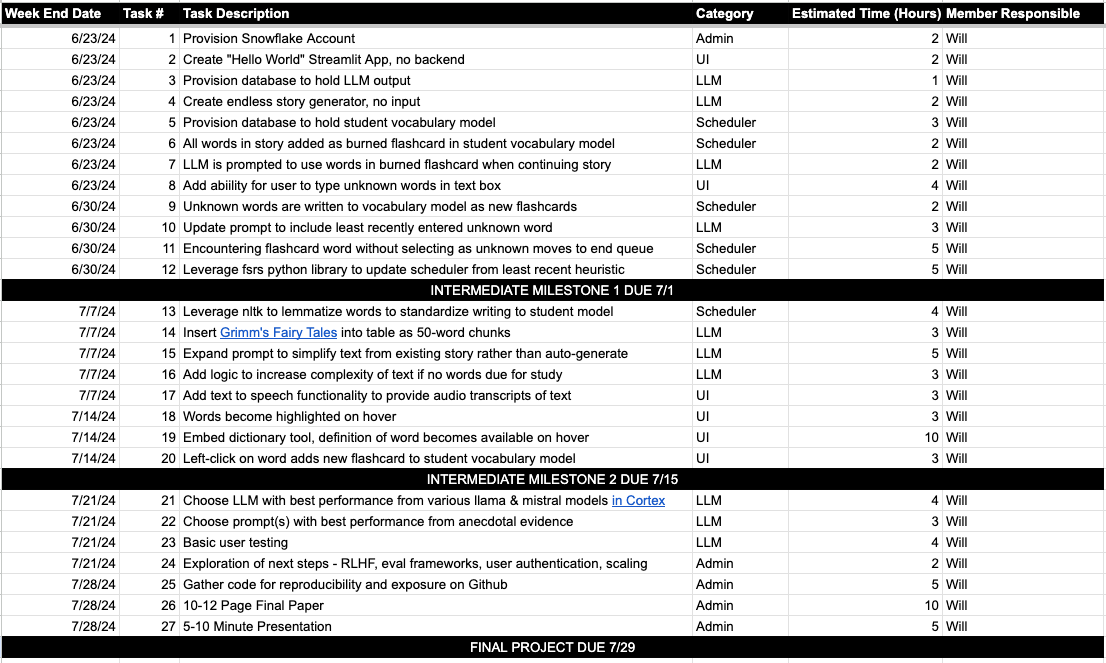
\includegraphics[width=0.9\linewidth]{Project Proposal/project_plan.png}
    \caption{Also available \href{https://docs.google.com/spreadsheets/d/10IeplrSFJeub_BLcY34Mex57YlT-x3DftFnladG2l4g/edit?usp=sharing}{here}}
    \label{Task List}
\end{figure}

\printbibliography{}

\end{document}

